\documentclass[fontsize=10pt,paper=b5,open=any,
twoside=no,toc=listof,toc=bibliography,headings=optiontohead,
captions=nooneline,captions=tableabove,english,DIV=15,numbers=noenddot,final,parskip=yes,
headinclude=true,footinclude=false,BCOR=0mm]{scrartcl}
\pdfvariable suppressoptionalinfo 512\relax
\synctex=1

\author{Valentin Boettcher, Bill Coish}
\usepackage{hirostyle}
\usepackage{hiromacros}
\addbibresource{references.bib}

\title{The non-Markovian Quantum Walk for Finite Baths (Summary)}
\date{\today}
\graphicspath{{plots}}


\begin{document}
\maketitle
In this report we reproduce the phase diagram obtained in
\refcite{Ricottone2020}. In \refcite{Ricottone2020} an infinite
reservoir and vanishingly small coupling was assumed. Here, in
contrast, we consider a finite number \(N\) reservoir states and a
finite coupling strength. The final result is presented in
\cref{fig:example_finite_vs_continuum} for \(N=50\) states. For the
correct choice of coupling strength, \(N=50\) reservoir levels are
likely not even necessary. We expect to see a reasonable reproduction
of the phase diagram even for a more modest number of reservoir
levels, satisfying \(N\gg 1\).

\begin{figure}[H]
  \centering
  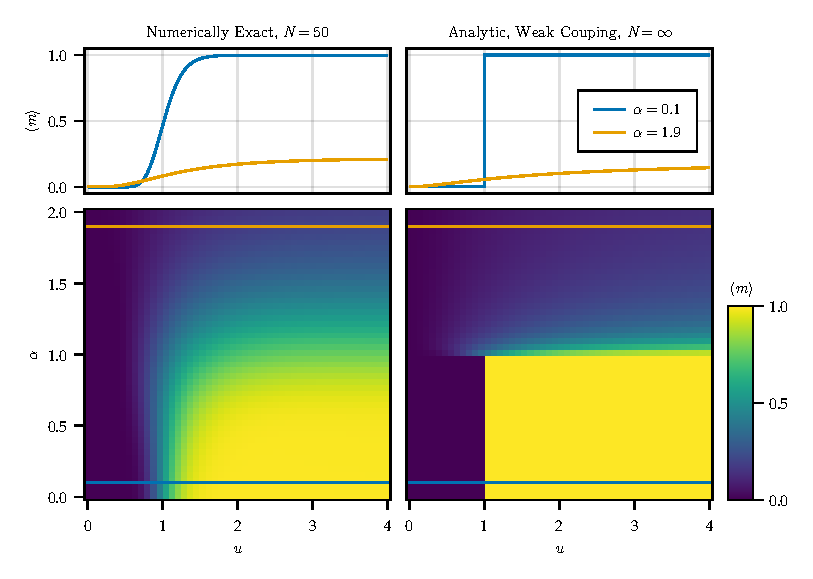
\includegraphics{plots/example_finite_vs_continuum}
  \caption{\label{fig:example_finite_vs_continuum} The full phase
    diagram and constant-\(α\) cuts obtained through numerical
    diagonalization for \(N=50\) reservoir modes (left) and through an
    analytic calculation in the weak-coupling limit (right) for
    \(N\to ∞\). All plots shown assume a coupling strength of
    \(g_{0}=0.2 ω_{c}\). Here, \(\ev{m}\) is the long-time
    time-averaged walker displacement, \(u=v\prime/v\) is the ratio of
    the inter-cell to intra-cell hopping amplitudes of the underlying
    SSH model, and \(α\) characterizes the bath spectral density at
    low frequency, \(J(ω)\sim ω^{α}\). We used \cref{eq:66} to adjust
    the energy \(ω_{A}\) of the \(A\) site to compensate for level
    repulsion.}
\end{figure}

The basic model is given by~\cite{Ricottone2020}
\begin{align}
  \label{eq:58}
  H &= H_{A} +H_{\bar{A}} + V\\
  H_{A} &= ∑_{m=0}^{L-1}ε_{A} a_{A,m}^{†}a_{A,m} \\
  H_{\bar{A}} &= ∑_{m=0}^{L-1}{(ε_{A} + ω)a_{B,m}^{†}a_{B,m}}+
                   ∑_{j=1}^{N}\bqty{ε_{j} b_{j,m}^{†}b_{j,m} + g_{j}
                   \pqty{a_{B,m}^{†}b_{j,m} + \hc}}\\
  V&=∑_{m=0}^{L-1} v\pqty{a_{A,m}^{†}a_{B,m}+ u a_{A,m}^{†}a_{B,m+1}} + \hc,
\end{align}
which describes an SSH chain with \(L\) sites, periodic boundary
conditions, intra-cell hopping amplitude \(v\) and inter-cell hopping
amplitude \(v\prime = u\cdot v\). The energy of each \(B\) site is
detuned from the \(A\)-site energy \(ε_{A}\) by the detuning
\(ω\). Further, we add \(N\) extra ``reservoir'' modes \(b_{j,m}\)
with energies \(ε_{j}\) in each unit cell. Those modes are then
coupled to the \(B\)-site in the unit cell via coupling strengths
\(g_{j}\). We are using second quantized notation here, where
\(a^{†}_{X,m}\ket{0} = \ket{X,m}\) creates a particle at sublattice
site \(X\) and lattice site \(m\), and
\(b^{†}_{j,m}\ket{0} = \ket{j,m}\) creates a particle in the \(j\)th
reservoir mode at site \(m\). The \(a\) and \(b\) operators obey the
usual bosonic commutation relations. This is equivalent to the
single-particle picture in \refcite{Ricottone2020}, as this
Hamiltonian preserves excitations.

We are interested in the evolution of a particle on the laltice, the
``walker'', that is initially localized to one \(A\) site
\(\ket{\psi(0)}=\ket{A,0}\).  The crucial observable is
\begin{equation}
  \label{eq:59}
  \ev{m(t)} \equiv ∑_{m}m {ρ_{\bar{A},m}(t)},
\end{equation}
where
\(ρ_{\bar{A},m}(t) = {∑_{l\neq A} \abs{\braket{l,m}{ψ(t)}}^{2}}\) is
the probability that the walker does reside in cell \(m\) but not on
the \(A\) site at time \(t\).  The long-time average of \(\ev{m(t)}\)
is sensitive to the topological phase of the bare SSH
model\footnote{This is understood as setting \(g_{j}=0\) and \(ω=0\)
  leaving \(v\) and \(u\) unchanged.}.  This phase is controlled by
the parameter \(u\) and the time averaged value of \(\ev{m(t)}\) will
reach a universal value indicating the topological phase, depending on
the structure of the reservoir, namely the choice of the energies
\(ε_{j}\) and the couplings \(g_{j}\).

To simplify calculations, we exploit the translational symmetry of the
model to express it in momentum space and remove the \(B\) sites by a
Schrieffer-Wolff transformation for large detuning \(ω\) resulting in
\(H=∑_{k}H(k)\) with
\begin{equation}
  \label{eq:61}
  H(k) = {ω}_{A} a_{A,k}^{†}a_{A,k}+ ∑_{j} \bqty{{ω}_{j} b_{j,k}^{†}b_{j,k}
    + \pqty{\frac{v(k)}{\abs{v(0)}}η_{j} a_{A,k}^{†}b_{j,k}+ \hc}},
\end{equation}
where \(k=\frac{2π n}{L}\) for \(n\in[0, L-1]\), \(L\in\NN_{>0}\) is the
number of lattice sites,
\(c_{l,k} = \frac{1}{\sqrt{L}}∑_{m}c_{l,m}\eu^{-\iu k m}\) and
\begin{equation}
  \label{eq:72}
  v(k)=v+v\prime\eu^{\iu k}=v\pqty{1+u\eu^{\iu k}} = \abs{v(k)}\eu^{\iu ϕ(k)}.
\end{equation}


The mean displacement can be re-expressed in terms of momentum-space quantities
\begin{equation}
  \label{eq:62}
  \begin{aligned}[t]
  \ev{m(t)} &= ∑_{k} \pqty{\frac{1}{L}-ρ_{A}\pqty{k,
              t}}\dv{ϕ({k})}{k}
  \end{aligned}
\end{equation}
where
\(ρ_{A}(k,t)=\pqty{L^{-1}-ρ_{\bar{A}}(k,t)}=\abs{\braket{A,k}{ψ(t)}}^{2}\)
with \(\ket{ψ(0)}=\sqrt{L^{-1}}∑_{k}\ket{A,k}=\sqrt{L^{-1}}∑_{k}a^{†}_{A,k}\ket{0}\).

The structure of the reservoir is described by the
spectral density, which we choose to take the form of a power law
\begin{equation}
  \label{eq:64}
  J(ω)
  =
  \begin{cases}
    {g_{0}^{2}\frac{(α+1)}{ω_{c}^{α+1}}} ω^{α} & \mathrm{for}\; 0\leq
                                               ω\leq ω_{c}\\
    0 & \mathrm{otherwise},
  \end{cases}
\end{equation}
where \(ω_{c}\) is called the cutoff frequency and \(α\) controls how
fast \(J(ω)\) approaches zero for \(ω\to 0\). The coupling strength
\(g_{0}\) can be expressed in terms of the couplings to the bath levels
\begin{equation}
  \label{eq:70}
  g_{0} = \sqrt{∑_{j}\abs{η_{j}}^{2}}.
\end{equation}
For finite-size reservoirs, a simple choice for the \(ω_{j}\) and
\(η_{j}\) is
\begin{equation}
  \label{eq:65}
  \begin{aligned}
    Δω &= \frac{ω_{c}}{N} & ω_{j} &= Δω \pqty{j + \frac{1}{2}} & η_{j}^{2}
    &= J(ω_{j}) Δω,
  \end{aligned}
\end{equation}
which recovers \cref{eq:64} in the limit \(N\to ∞\).

The finite size of the reservoir will in general wash out the sharp
phase transitions observed in \refcite{Ricottone2020}. Additionally, it
will lead to recurrences in the dynamics around the time
\begin{equation}
  \label{eq:71}
  τ_{R}=\frac{2π}{Δω},
\end{equation}
as is illustrated in \cref{fig:mean_displacement_example}.
\begin{figure}[H]
  \centering
  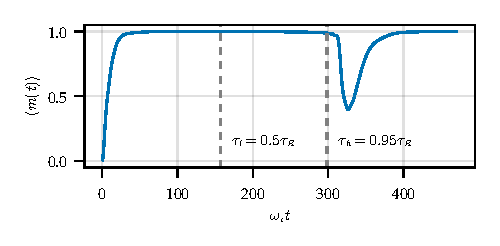
\includegraphics[width=.8\linewidth]{plots/mean_displacement_example_simple}
  \caption{\label{fig:mean_displacement_example} The mean displacement
    \(\ev{m(t)}\) over time for \(g_{0}=0.2 ω_{c}\), \(α=0.1\),
    \(u=4\), \(N=50\). The interval for the time average in
    \cref{eq:69} used in \cref{fig:example_finite_vs_continuum} is
    visualized by the dashed vertical lines.}
\end{figure}

Also, the mean displacement decays to a steady state
approximately\footnote{Obtained through the golden rule using a flat,
  continuous bath spectrum.} with a rate
\begin{equation}
  \label{eq:1}
  Γ = \frac{π g_{0}^{2}}{ω_{c}}.
\end{equation}
It is therefore necessary to separate the time scale of transient
dynamics \(1/Γ\) from the time scale of recurrences \(τ_{R}\) so that
\(1/Γ \ll τ_{R}\), which gives a lower bound for the number of
reservoir states required given a coupling strength
\begin{equation}
  \label{eq:73}
  N \gg \frac{ω_{c}^{2}}{2π^{2}g_{0}^{2}}.
\end{equation}

Further, there exists a limit of strong coupling, where
\(\ev{ρ_{A}(k, t)}\sim \cos[2](Ω t)\) with
\(Ω=\sqrt{∑_{j}\abs{η_{j}}^{2}}\).  As this limit leads to persistent
oscillations rather than the behavior of
\cref{fig:example_finite_vs_continuum} it has to be avoided by
choosing
\begin{equation}
  \label{eq:2}
  g_{0} \ll ω_{c}.
\end{equation}
The balance has to be kept between the number of reservoir states
required for the separation of time scales \(N\sim g_{0}^{-2}\) and
avoiding the strong-coupling limit.

We now define the time-averaged mean displacement as
\begin{equation}
  \label{eq:69}
  \ev{m} \equiv \frac{1}{τ_{h} - τ_{l}} ∫_{τ_{l}}^{τ_{h}}\ev{m(t)} \dd{t},
\end{equation}
with \(τ_{l}\) and \(τ_{h}\) chosen appropriately to avoid transient
behavior on time scales of the order of \(1/Γ\) and recurrences at
\(τ_{R}\), but far enough apart to provide a satisfactory
average. Here we choose \(τ_{l}=0.5 τ_{R},\, τ_{h} = 0.95 τ_{R}\), as
is visualized in \cref{fig:mean_displacement_example}.

In the continuum limit revivals won't occur, so that we can take the
limit of \(τ_{h}\to ∞\) and \(τ_{l}=0\) obtaining
\begin{equation}
  \label{eq:60}
  \ev{m} =  \lim_{T\to ∞} \frac{1}{T} ∫_{0}^{T}\ev{m(t)}\dd{t}.
\end{equation}
If \(ρ_{A}(k,t)\xrightarrow{t\to ∞}0\) for all \(k\), the long-time
averaged mean displacement \(\ev{m}\) exhibits a universal behavior
corresponding to the topological phase of the original SSH chain
\begin{equation}
  \label{eq:63}
  \ev{m} = θ(u-1).
\end{equation}
In \refcite{Ricottone2020}, an infinite SSH chain (\(L=∞\)) was
studied within the Born approximation and in the continuum limit for
the reservoir. There, it was found that \(\ev{m}\) matches
\cref{eq:63} precisely for \(α<1\), whereas it takes on non-universal
values for \(α>1\). This behavior can also be obtained without
employing the Born approximation and is presented in the right column
of \cref{fig:example_finite_vs_continuum}.

If we choose \(ω_{c}=1\) (choice of units) and \(g_{0}=0.2 ω_{c}\), we
avoid the strong-coupling behavior \cref{eq:2}, while the criterion
for the separation of time scales in \cref{eq:73} becomes
\begin{equation}
  \label{eq:3}
  N\gg \frac{100}{8π^{2}} \approx 1.27.
\end{equation}
This estimate suggests that, for this choice of coupling, we should
expect to have a region in time of ``universal'' saturation in
\(\ev{m(t)}\) whenever \(N\gg 1\), thus reproducing the key feature of
the phase diagram.  The resulting \(\ev{m(t)}\) for \(N=50\),
\(α=0.1\), and \(u=4\) is shown in
\cref{fig:mean_displacement_example}, where we see that the time
scales are indeed well separated and \(\ev{m}\approx 1\) as was also
found in the continuum limit (\(N\to ∞\)) and for weak coupling.

When choosing a moderately large \(g_{0}\) and finite \(N\) we have to
compensate for level repulsion which shifts the effective energy of
the \(A\)-site.  This effect can be countered by choosing a specific
value of the \(A\)-site energy
\begin{equation}
  \label{eq:66}
  ω_{A} = ∑_{j}\frac{\abs{η_{j}}^{2}}{ω_{j}} = ∑_{j}
  J(ω_{j}) \frac{Δω}{ω_{j}},
\end{equation}
where \(ω_{A}\) is independent of \(u\), but still depends on
\(α\). \Cref{fig:mean_displacement_example} was produced in this way.

The full phase diagram for the finite reservoir is presented on the
left side of \cref{fig:example_finite_vs_continuum}. While finite-size
effects wash out the sharp borders of the phase diagram, its signature
is relatively clear, especially in the constant-\(α\) cuts above the
phase diagram.

\printbibliography{}
\end{document}


%%% Local Variables:
%%% mode: latex
%%% TeX-master: t
%%% TeX-output-dir: "output"
%%% TeX-engine: luatex
%%% End:
